\section{Fault Modeling and the Safety Annex}
\label{sec:fault_modeling}

\subsection{Features needed for fault modelling}
It is assumed that an AADL model of the nominal system specifies the hardware, software, and mechanical components of the system and their interconnections. This model is annotated with behavioral contracts using the AGREE annex~\cite{NFM2012:CoGaMiWhLaLu}. The nominal model behavioral requirements are verified using inductive model checking through AGREE~\cite{2017arXiv171201222G}. At this point, the fault modelling can commence. 

%The usage of the terms error, failure, and fault are defined in ARP4754A and are described here for ease of understanding~\cite{SAE:ARP4754A}. A \textit{failure} is an event that occurs when the delivered service of a system deviates from correct behavior. A service of a system is a sequence of the system's external states. This deviation from correct behavior is called an \textit{error}. The cause of an error is a \textit{fault}. Faults can be \textit{active} or \textit{dormant}. A fault is active when it causes an error to occur, else it is dormant. We use {\em fault} as the generic modeling keyword throughout the AADL model hierarchy and follow the definitions of these terms throughout this description. 

When conducting the safety assessment and examining the individual subcomponents of a system, the faults and failure modes must be determined. A fault is the manifestation of an error that may lead to failure in a given component~\cite{SAE:ARP4754A}. For example, a fault in a valve may be that it is stuck closed. If this fault is active, it may cause a failure to occur. If there is no command to provide outgoing pressure, then this active fault will not cause a failure of the component to perform as intended. On the other hand, if there is such a command to provide pressure, this fault will cause failure of the valve component. The failure mode in this case is that there is a command to provide outgoing pressure, but an active fault on the valve causes it to be stuck closed. 

Many of these modes can be determined through domain knowledge and other modes are specified through the manufacturer of a given mechanical or digital component. Once the faults and failure modes are determined, the safety engineer must determine the consequence of this component failure on connected components, components that are physically located nearby, or on the system as a whole. Given that many safety critical systems are quite complex, this propagation process can be error prone and time consuming.

In the following subsections, we walk through examples of component failure modes to illustrate how a safety engineer can use the Safety Annex to perform these assessments and see how an active fault may or may not cause failure of a component.

Once the system level functions and results of the FHA have been determined, these are used to guide the architecture development of the system. This process normally starts early in the development life cycle and is quite iterative in nature~\cite{AIR6110}. Following the example described in Section~\ref{sec:case_study} and outlined in AIR6110, we describe the process of integrating this fault modeling process into the iterative processes given in AIR6110. 

In the AADL system model and the AGREE behavioral model, we have the component structures and behaviors (properties) defined for the system subcomponents. Assuming that the nominal model holds, i.e. in the absence of faults, the system behavior is sound, it is of interest to see how the presence of faults affect the overall system functionality. To determine this information, a safety engineer must determine what possible faults could be present in the given components of the system. 

\subsection{Failure modes of a digital component}

The WBS model contains a wide variety of components ranging from digital to mechanical. Using the Safety Annex, it is possible to capture a variety of fault descriptions for these components. As described in Section~\ref{sec:case_study}, one of the components important to the property \textit{Inadvertant braking}, is the pedal. When the mechanical pedal is pressed, a sensor reads this information and passes an electronic signal to the BSCU which then proceeds in commanding hydraulic pressure to the wheels. 

\begin{figure}[h!]
	\hspace*{-2cm}
	\vspace{-0.5in} 
	\begin{center}
		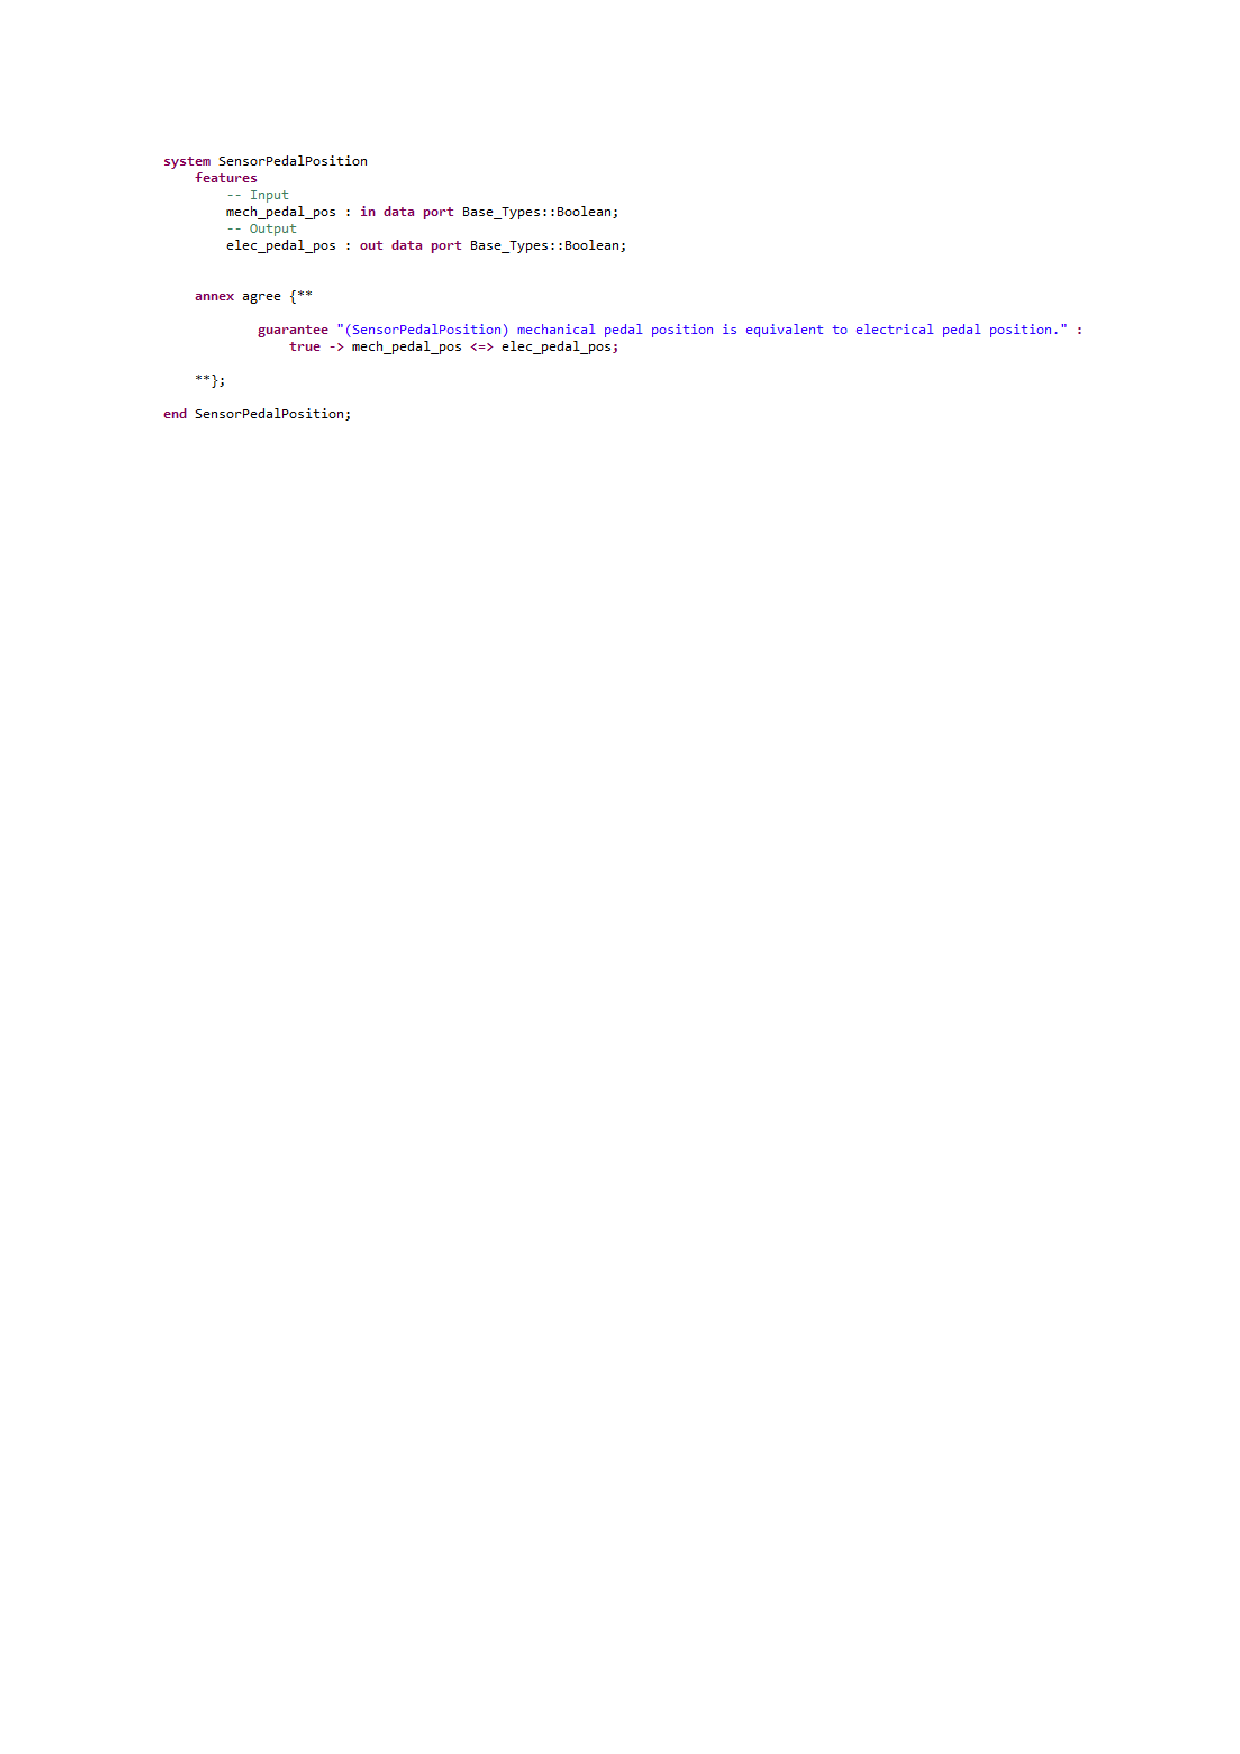
\includegraphics[trim=0 640 -10 70,clip,width=1.5\dimexpr\textwidth-2cm\relax]{images/sensorPedalAADL.pdf}
		\caption{An AADL System Type: The Pedal Sensor}
		\label{fig:sensor}
	\end{center}
	%\vspace{-0.4in}
\end{figure}

 In Figure~\ref{fig:sensor}, the AADL system component is shown with a contract on the output of this component. The sensor has only one input: the mechanical pedal position and one output: the electrical pedal position. The property that governs the behavior of the component is that the mechanical position should always equal the electronic position. This is an example of the nominal system model in AADL with behaviors defined in AGREE. 

\begin{figure}[h!]
	\hspace*{-2cm}
	\vspace{-0.5in} 
	\begin{center}
		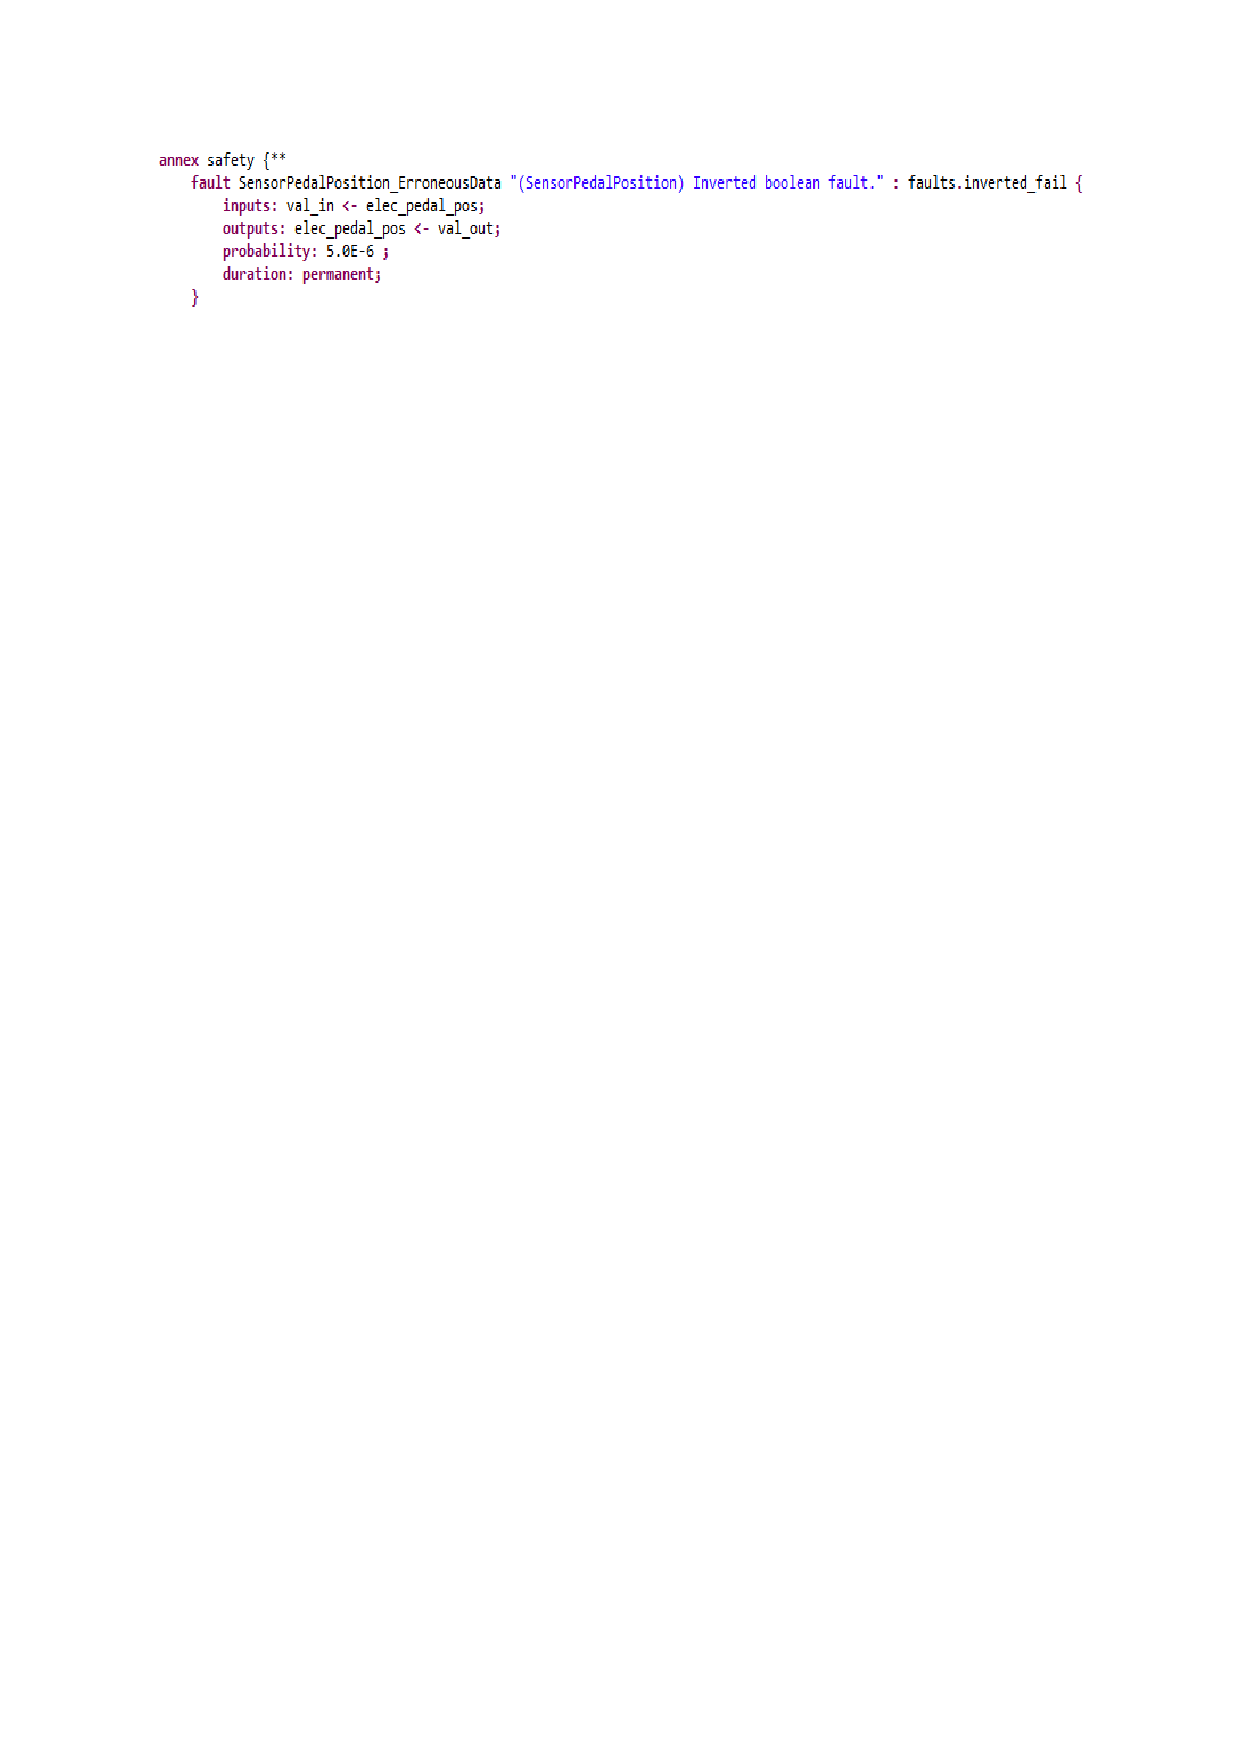
\includegraphics[trim=0 690 -10 70,clip,width=1.5\dimexpr\textwidth-2cm\relax]{images/sensorPedalFault.pdf}
		\caption{The Safety Annex for the Pedal Sensor}
		\label{fig:sensorFault}
	\end{center}
	%\vspace{-0.4in}
\end{figure}

This sensor has a known fault which can invert the signal read and pass along an incorrect value. This fault is known to occur with probability $5.0e-6$. In Figure~\ref{fig:sensorFault}, the Safety Annex definition for this particular fault is shown. The faults are defined using a library of fault nodes (in this case, \textit{inverted\_fail}) and when the fault is triggered, the output of the component is converted into its failure value. 

\iffalse

The \textit{fault statement} consists of a unique description string, the fault node definition name, and a series of \textit{fault subcomponent} statements. \\
\textbf{Inputs} in a fault statement are the parameters of the fault node definition. In the example above, \textit{val\_in} and \textit{alt\_val} are the two input parameters of the fault node. These are linked to the output from the Pump component (\textit{pressure\_output.val}), and \textit{alt\_value}, a fail to value of zero. When the analysis is run, these values are passed into the fault node definition.\\
\textbf{Outputs} of the fault definition correspond to the outputs of the fault node. The fault output statement links the component output (\textit{pressure\_output.val}) with the fault node output (\textit{val\_out}). If the fault is triggered, the nominal value of \textit{pressure\_output.val} is overridden by the failure value output by the fault node. Faulty outputs can take deterministic or non-deterministic values. \\
\textbf{Probability} (optional) describes the probability of a fault occurrence.\\
\textbf{Duration} describes the duration of the fault; currently the Safety Annex supports transient and permanent faults.\\

\fi

\subsection{Error propagation of the pedal sensor failure}

When this particular fault is active in the system, we can run the analysis to see how it propagates through the system. The classification of the top level safety property is catastrophic and carries a probability threshold of $1.0e-9$. Upon running the fault analysis in the toolset, a counterexample is provided for this top level property given the fault definition provided in Figure~\ref{fig:sensorFault}. Since the probability of this fault occuring on the sensor is higher than that of the top level property, it is of interest. 

Through the counterexample display we can trace the behavior of the system when this particular fault is active. The mechanical pedal is not pressed, but this failure causes the sensor subcomponent to report to the BSCU that it was pressed. The active BSCU channel uses this value in order to command braking, determine validity of the channel and control the antiskid behavior of the aircraft. The BSCU carries on with its normal behavior assuming that the pedal was pressed and the state of the system is as follows: braking is not commanded and power is supplied throughout the system. The ground is moving, there is braking force at the wheels, and the wheel is rolling. Taken together this clearly disproves the top level contract that inadvertant braking at a given wheel does not occur. Thus the safety analyst of this system can recognize that some set of precautions are required for the pedal sensor component. 

\subsection{Failure modes of a mechanical component}
In the WBS there are a number of mechanical components which include valves, pumps, and wheels. When finding the failure modes of, for example, a valve, we must be aware of the ways a valve can fail. It can be stuck completely open, stuck closed, or somewhere in between. Of course this ``somewhere in between'' value could be the previous position of the valve or it could be a nondeterministic value between open and closed. For the valves in the WBS all of these possible faults can be defined through the use of separate fault statements (a complete fault statement is defined in Figure~\ref{fig:sensorFault}). 


\subsection{Hardware failure modes} 
There is another set of possible failures in a system that are difficult to capture with the fault definitions previously discussed. As described in Section~\ref{subsec:comparison_with_EMV2}, explicit fault propagation is something that currently exists in EMV2 for AADL, but there are cases when the occurrence of an event can cause a chain reaction and trigger other faults to occur. For example, the pumps are stored in the same physical location and a fire breaks out in that room. Or a processor overheats which causes an adjacent processor to do the same. It is desirable to model these faults and one must be able to identify which component failures are activated due to the unfortunate occurrance. To this end, the Safety Annex has the ability to define what is called a Hardware fault and the user then must define which component faults are triggered by this one active fault. 

As an example, consider if the green hydraulic pump and the blue pump are stored adjacent and something happens to cause the blue pump to explode. The effect of this mishap causes the blue pump to no longer output pressure and it triggers the adjacent pump to do the same.  
















\iffalse


\danielle{Leaving the rest of this for now so that I can easily pull from it if need be.}


In this section, we describe the main features and functionality of the Safety Annex. The usage of the terms error, failure, and fault follow their definitions in ARP4754A~\cite{SAE:ARP4754A}. We use {\em fault} as the generic modeling keyword throughout the AADL model hierarchy.

\subsection{Basic Functionality}

An AADL model of the nominal system behavior specifies the hardware and software components of the system and their interconnections. This nominal model is then annotated with assume-guarantee contracts using the AGREE annex~\cite{NFM2012:CoGaMiWhLaLu} for AADL. The nominal model requirements are verified using compositional verification techniques based on inductive model checking~\cite{2017arXiv171201222G}.

Once the nominal model behavior is defined and verified, the Safety Annex can be used to specify possible faulty behaviors for each component. The faults are defined on each of the relevant components using a customizable library of fault nodes and the faults are assigned a probability of occurrence. A probability threshold is also defined at the system level. This extended model can be analyzed to verify the behavior of the system in the presence of faults. Verification of the nominal model with or without the fault model is controlled through the safety analysis option during AGREE verification.

To illustrate the syntax of the Safety Annex, we use an example based on the Wheel Brake System (WBS) described in ~\cite{AIR6110} and used in our previous work ~\cite{Stewart17:IMBSA}.
The fault library contains commonly used fault node definitions. An example of a fault node is shown below:
\begin{figure}[h!]
	\hspace*{-4cm}
	\vspace{-0.5in} 
	\begin{center}
		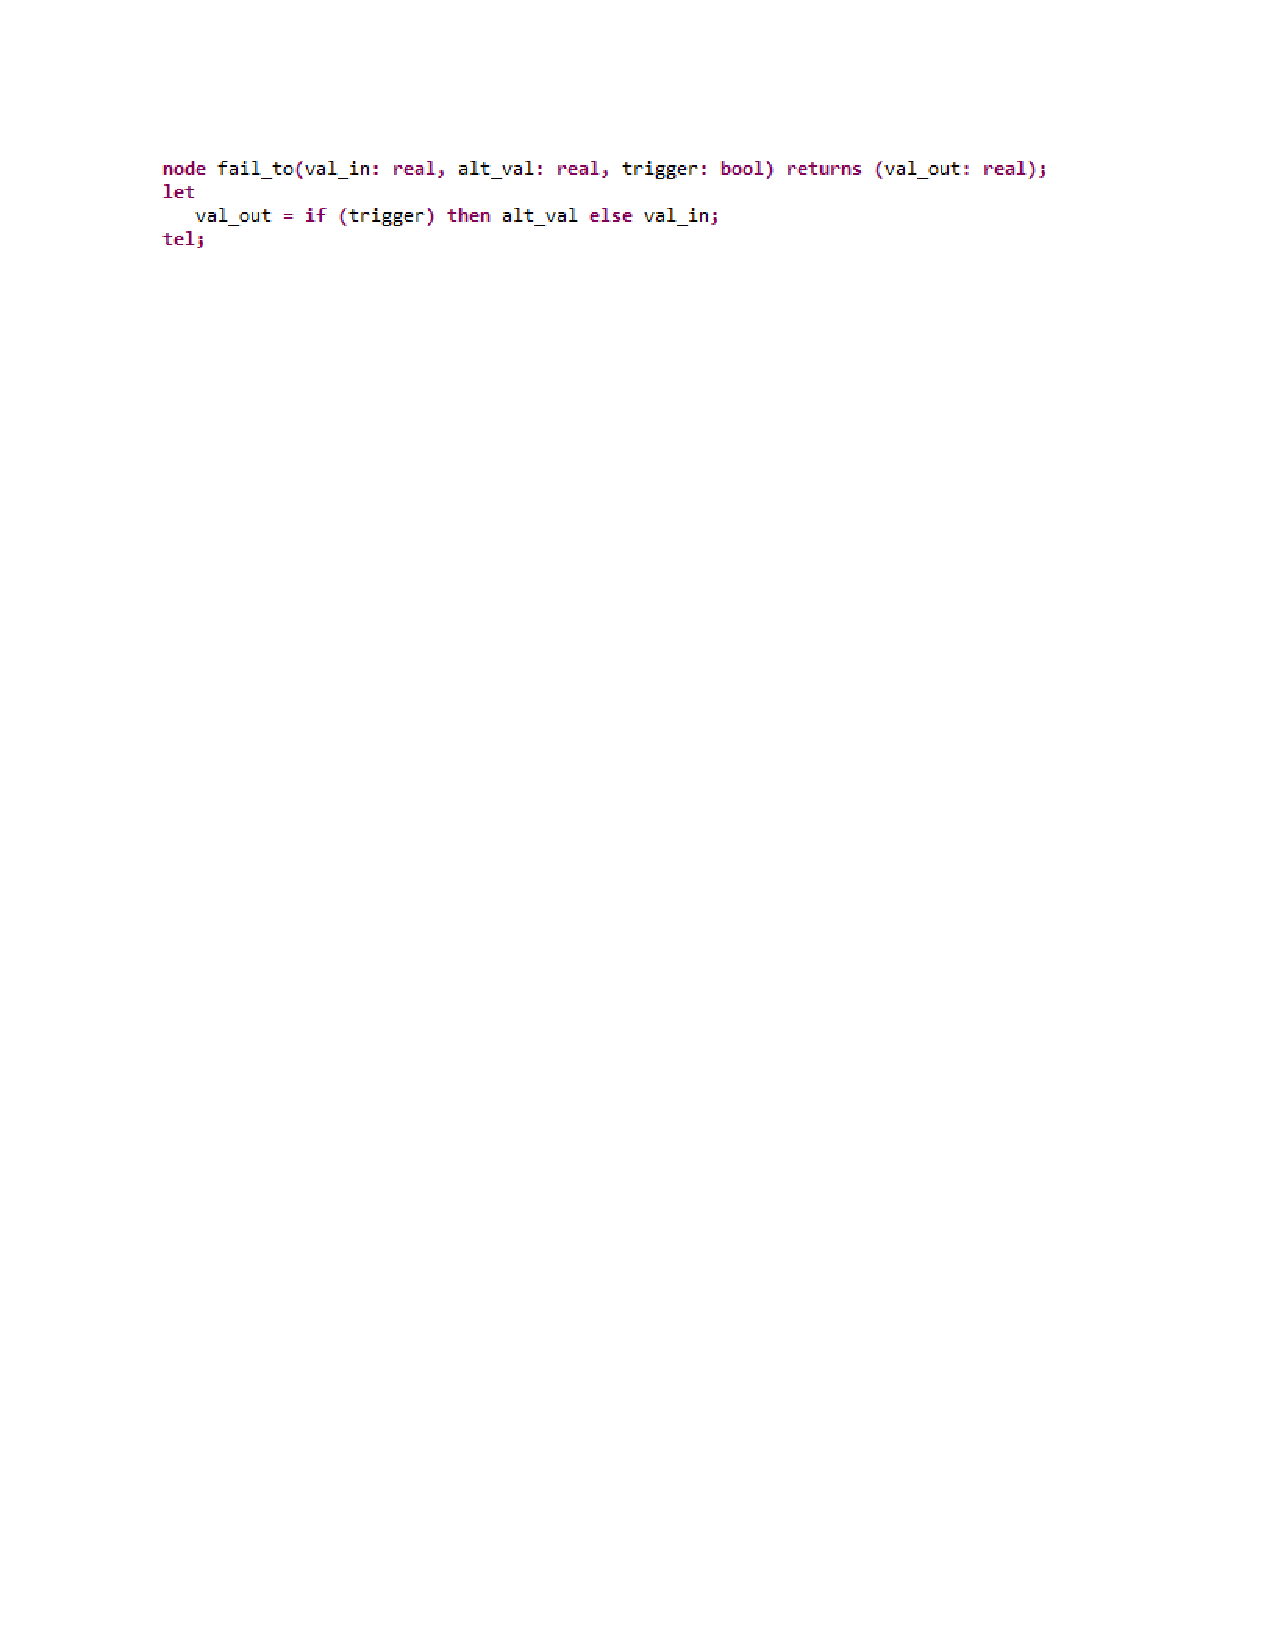
\includegraphics[trim=0 670 -10 70,clip,width=1.3\dimexpr\textwidth-1.5cm\relax]{images/fault_node.pdf}
	\end{center}
	\vspace{-0.4in}
\end{figure}

The \textit{fail\_to} node provides a way to inject a faulty input value. When the \textit{trigger} condition is satisfied, the nominal component output value is overridden by the \textit{fail\_to} failure value. In the WBS, the pump component generates an expected amount of pressure to a hydraulic line.  Declaration of a fail to zero fault in the pump component is shown below:
\begin{figure}[h!]
	\hspace*{-3cm} 
	\vspace{-0.6in}
	\begin{center}
		%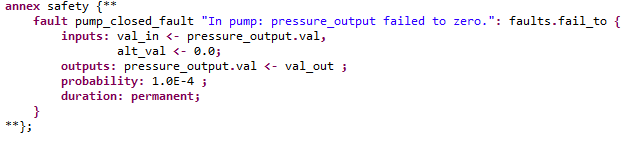
\includegraphics[trim=0 330 150 0,clip,width=1.0\textwidth]{images/pump_fault.png}
		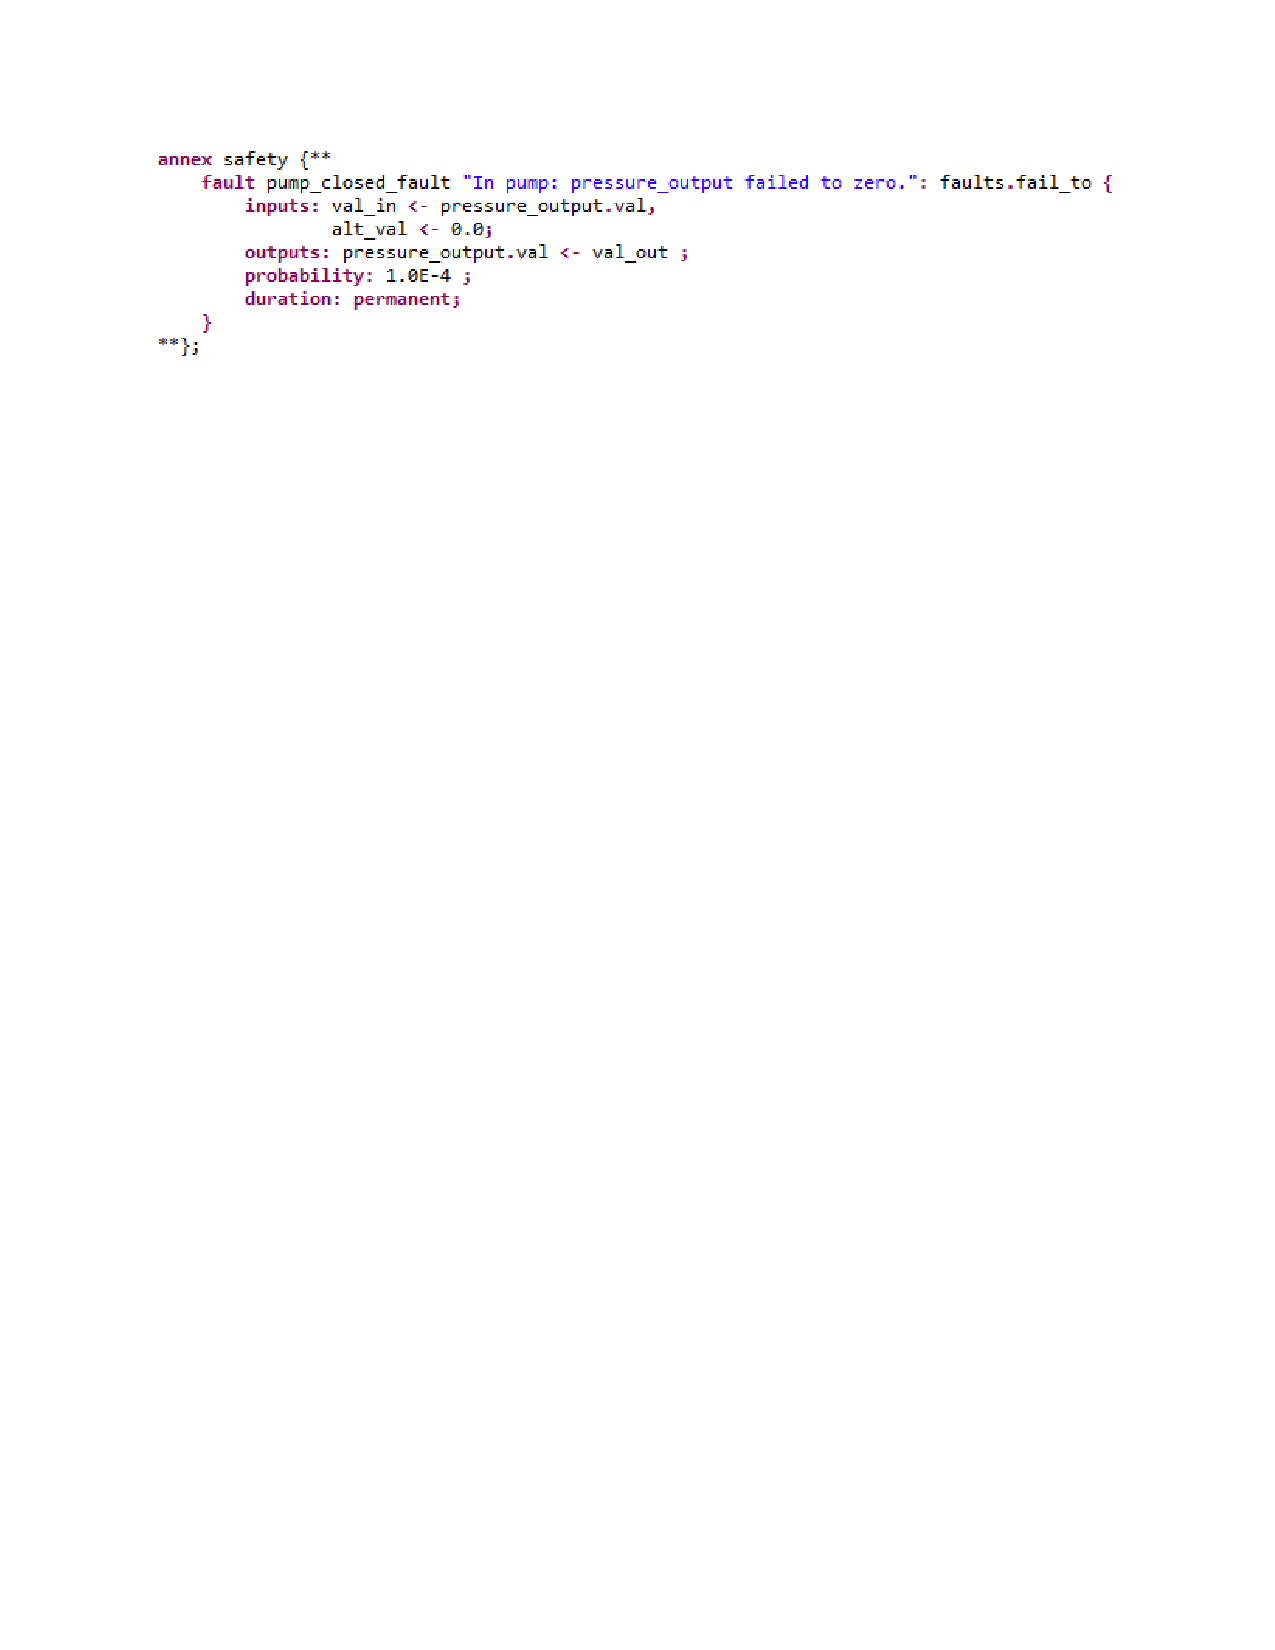
\includegraphics[trim=60 620 0 60,clip,width=1.3\dimexpr\textwidth-1.5cm\relax]{images/pump_fault.pdf}
	\end{center}
	\vspace{-0.40in}
\end{figure}

The \textit{fault statement} consists of a unique description string, the fault node definition name, and a series of \textit{fault subcomponent} statements. \\
\textbf{Inputs} in a fault statement are the parameters of the fault node definition. In the example above, \textit{val\_in} and \textit{alt\_val} are the two input parameters of the fault node. These are linked to the output from the Pump component (\textit{pressure\_output.val}), and \textit{alt\_value}, a fail to value of zero. When the analysis is run, these values are passed into the fault node definition.\\
\textbf{Outputs} of the fault definition correspond to the outputs of the fault node. The fault output statement links the component output (\textit{pressure\_output.val}) with the fault node output (\textit{val\_out}). If the fault is triggered, the nominal value of \textit{pressure\_output.val} is overridden by the failure value output by the fault node. Faulty outputs can take deterministic or non-deterministic values. \\
\textbf{Probability} (optional) describes the probability of a fault occurrence.\\
\textbf{Duration} describes the duration of the fault; currently the Safety Annex supports transient and permanent faults.\\
%\textit{Equation Statements}: Equation statements support deterministic or nondeterministic types. For more details on equation statements, see ~\cite{NFM2012:CoGaMiWhLaLu}.
In addition, Safety Annex also supports the specification of faults without specific behaviors (e.g., hardware failures), and allows the explicit propagation between faults, to model the dependencies between hardware failures and system faults, or between different hardware failures.

\begin{comment}
\subsection{Hardware Failures and Dependent Faults}

Failures in hardware (HW) components can trigger behavioral faults in the software (SW) or system (SYS) components that depend on them.  For example, a CPU failure may trigger faulty behavior in threads bound to that CPU. In addition, a failure in one HW component may trigger failures in other HW components located nearby, such as cascading failure caused by a fire or water damage.

Faults propagate in AGREE as part of a system’s nominal behavior. This means that any propagation in the HW portion of an AADL model would have to be artificially modeled using data ports and AGREE behaviors in SW. This is less than ideal as there may not be concrete behaviors associated with HW components. In other words, faulty behaviors mainly manifest themselves on the SW/SYS components that depend on the hardware components.

To better model faults at the system level dependent on HW failures, we have introduced a new fault model element for HW components. In comparison to the basic fault statement introduced in the previous section, users are not specifying behavioral effects for the HW failures, nor data ports to apply the failure. An example of a model component fault declaration is shown below:
\begin{figure}[h!]
		\vspace{-0.2in}
	\begin{center}
		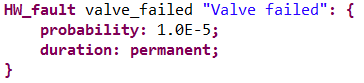
\includegraphics[width=.5\textwidth]{images/hw_fault.png}
	\end{center}
	\vspace{-0.4in}
\end{figure}

In addition, users can specify fault dependencies outside of fault statements, typically in the system implementation where the system configuration that causes the dependencies becomes clear (e.g., binding between SW and HW components, co-location of HW components). This is because fault propagations are typically tied to the way components are connected or bound together; this information may not be available when faults are being specified for individual components. Having fault propagations specified outside of a component’s fault statements also makes it easier to reuse the component in different systems. An example of a fault dependency specification is shown below, showing that the valve{\_}failed fault at the shutoff subcomponent triggers the pressure{\_}fail{\_}blue fault at the selector subcomponent.
\begin{figure}[h!]
	\vspace{-0.2in}
	\begin{center}
		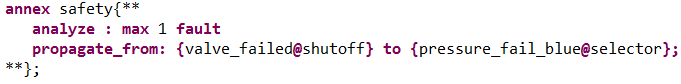
\includegraphics[width=.9\textwidth]{images/fault_propagation.png}
	\end{center}
	\vspace{-0.4in}
\end{figure}
\end{comment}

\subsection{Architecture and Implementation}

The architecture of the Safety Annex is shown in Figure~\ref{fig:plugin-arch}.  It is written in Java as a plug-in for the OSATE AADL toolset, which is built on Eclipse.  It is not designed as a stand-alone extension of the language, but works with behavioral contracts specified in AGREE AADL annex and associated tools~\cite{NFM2012:CoGaMiWhLaLu}.  AGREE allows {\em assume-guarantee} behavioral contracts to be added to AADL components.  The language used for contract specification is based on the Lustre dataflow language~\cite{Halbwachs91:IEEE}. AGREE improves scalability of formal verification to large systems by decomposing the analysis of a complex system architecture into a collection of smaller verification tasks that correspond to the structure of the architecture.

\begin{figure}
	\begin{center}
		%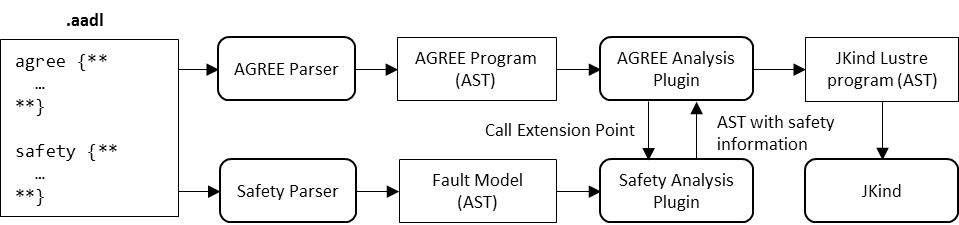
\includegraphics[trim=0 400 430 0,clip,width=0.85\textwidth]{images/arch.png}
		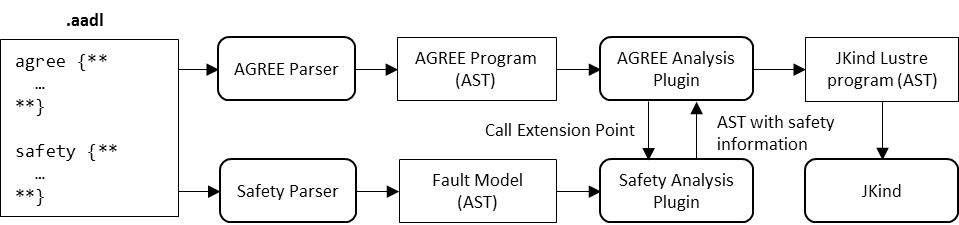
\includegraphics[width=.9\textwidth]{images/arch.png}
	\end{center}
	\vspace{-0.2in}
	\caption{Safety Annex Plug-in Architecture}
	\label{fig:plugin-arch}
\end{figure}

AGREE contracts are used to define the nominal behaviors of system components as {\em guarantees} that hold when {\em assumptions} about the values the component's environment are met.  The Safety Annex extends these contracts to allow faults to modify the behavior of component inputs and outputs.  To support these extensions, AGREE implements an Eclipse extension point interface that allows other plug-ins to modify the generated abstract syntax tree (AST) prior to its submission to the solver.  If the Safety Annex is enabled, these faults are added to the AGREE contract and, when triggered, override the nominal guarantees provided by the component.  An example of a portion of an initial AGREE node and its extended contract is shown in Figure~\ref{fig:comp}.  The \texttt{\_\_fault} variables and declarations are added to allow the contract to override the nominal behavioral constraints (provided by guarantees) on outputs.  In the Lustre language, \texttt{assertion}s are constraints that are assumed to hold in the transition system.

\begin{figure}
	\vspace{-0.1in}
	%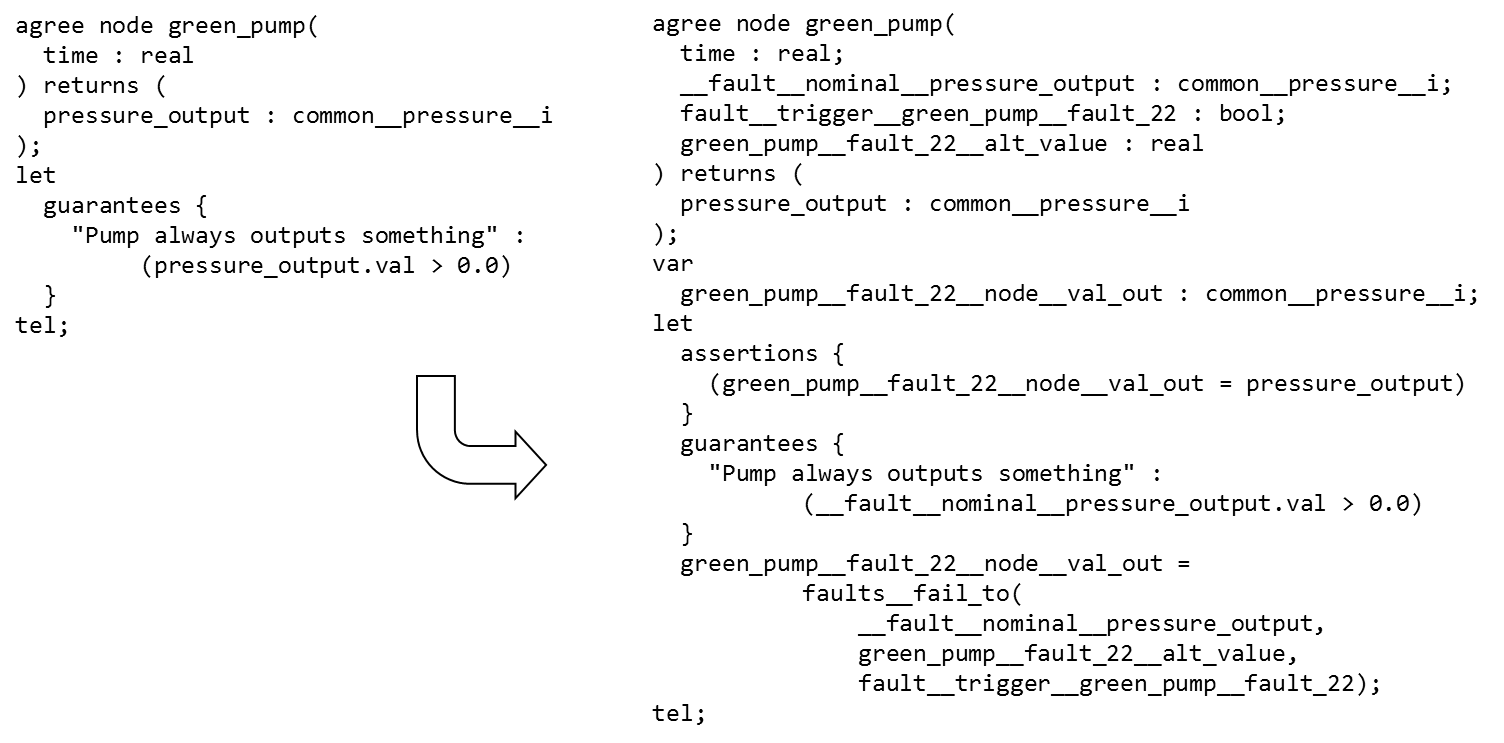
\includegraphics[trim=30 150 120 10,clip,width=\textwidth]{images/sample_code.png}
	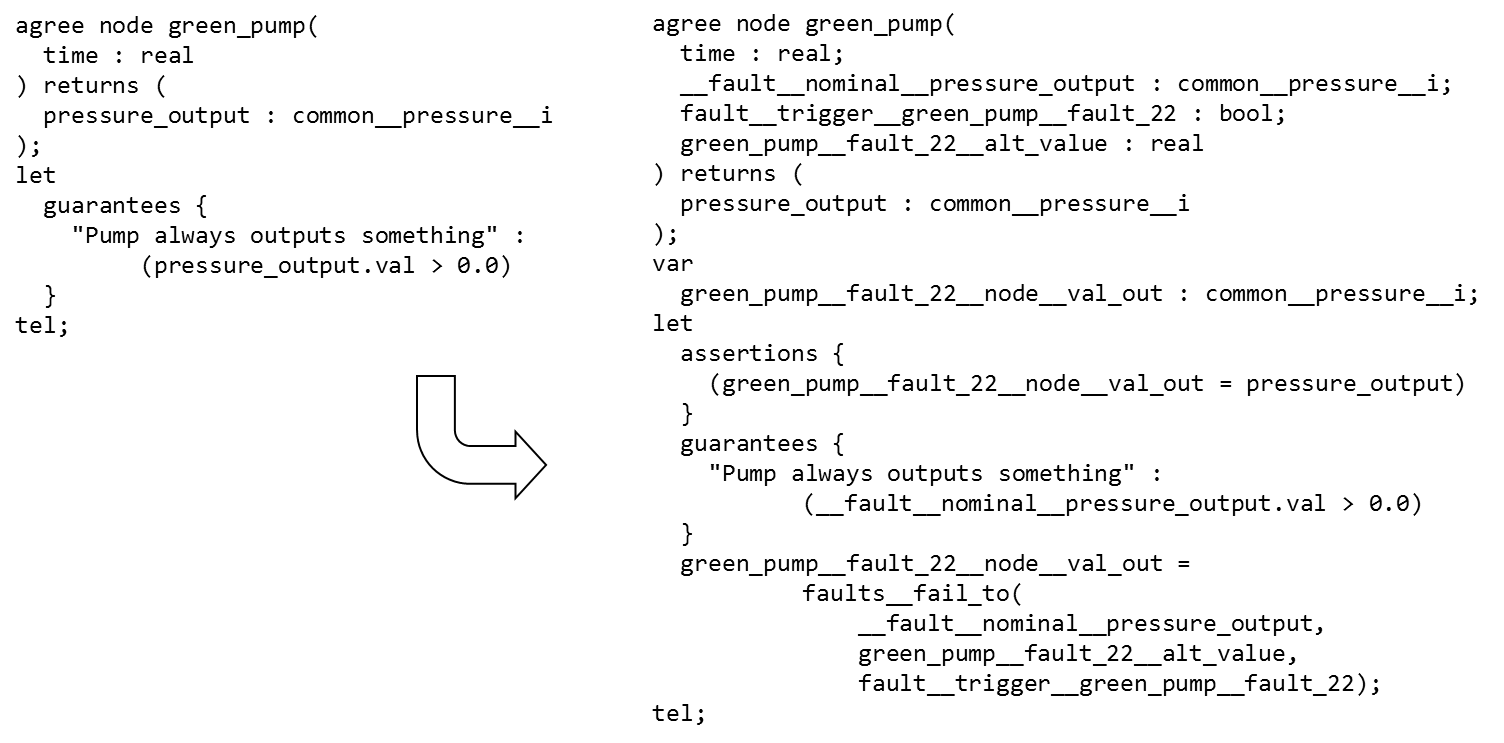
\includegraphics[width=\textwidth]{images/sample_code.png}
	\vspace{-0.3in}
	\caption{Nominal AGREE node and its extension with faults}
	\label{fig:comp}
\end{figure}

An annotation in the AADL model determines the fault hypothesis.  This may specify either a maximum number of faults that can be active at any point in execution (typically one or two), or that only faults whose probability of simultaneous occurrence is above some probability threshold should be considered. In the former case, we assert that the sum of the true {\em fault\_\_trigger} variables is below some integer threshold.  In the latter, we determine all combinations of faults whose probabilities are above the specified probability threshold, and describe this as a proposition over {\em fault\_\_trigger} variables.
%
With the introduction of dependent faults, active faults are divided into two categories: independently active (activated by its own triggering event) and dependently active (activated when the faults they depend on become active). The top level fault hypothesis applies to independently active faults. Faulty behaviors augment nominal behaviors whenever their corresponding faults are active (either independently active or dependently active).

Once augmented with fault information, the AGREE model follows the standard translation path to the model checker JKind~\cite{2017arXiv171201222G}, an infinite-state model checker for safety properties.  The augmentation includes traceability information so that when counterexamples are displayed to users, the active faults for each component are visualized.


%\subsection{Mapping to Safety Analysis Artifacts}

\begin{comment}
The following list describes how the basic safety concepts can be represented using the Safety Annex.

\begin{enumerate}
\item \textbf{Error} Definition and how we model it
\item \textbf{Fault} Definition and how we model it
\item \textbf{Failure} Definition and how we model it. Non deterministic faults
\item \textbf{Failure Mode}
\end{enumerate}


Errors/Faults/Failures - to a safety engineer, these terms have very specific meanings.  You will see my specific comments on this topic where I located them by your Section 3.3.  If needed, we can talk about this comment after I send you my mark-ups.
In Section 3.1, you introduce the term "non-deterministic".  I am not sure how your new process can be used by the safety engineering discipline unless things are "deterministic" and therefore "repeatable".
\end{comment}

\begin{comment}
A prerequisite of performing the safety assessment of a system design is to understand how the system works, primarily focusing on the integrity of the outputs and the availability of the product. The safety engineers then use the acquired understanding to conduct safety analysis, construct the safety analysis artifacts, and compare the analysis results with established safety objectives and safety related requirements.
%check Figure 7 of ARP-4754A for step by step process of the traditional approach
%How our approach can help: step by step process; inputs and outputs
%Drawback/inefficiencies with the current safety assessment
%The causal effect in the fault tree is manually come up by safety engineers after understanding the signal and function flow in the system/sw design documents for the related functionality.
%The logical causal relationship is represented in a descriptive fault tree structure.
%It works well when the signals are processed in a sequential/linear fashion, but not when there are interactions/feedback loops that make the causal effect no longer linear?

%case study
%AIR6110, Rockwell white paper
"working on safety analysis process. Strategy:
1. Check the example Mike Peterson did with stall warning
2. Come up with model in our end
3. See if we can catch anything missed by the fault tree, or help supply the fault tree analysis"
start process investigation by:
1. select the example from stall warning where mike has produced a fault tree from the document
2. independently model from the stall warning doc and try to:
get information from the fault tree that can build the structure of the fault tree
get information from the verification that can help trim/update the probability numbers of the fault tree
3. Compare the fault tree produced by Mike and the information supplied by our study, and see if we provide values to this study
Repeat this for an example fault tree from the white paper Mike sent

Process investigation
How should our model interact with the fault tree that Mike come up with? Any place we can work to create the tree for him? Or provide additional scenarios? Or validate the probabilities for his tree? Or SW/HW/Sys interactions that our approach captures that is hard to capture/verify using his approach?
How does the behavioral/interaction part of the document be modeled in the fault tree and in our model?
What findings from the safety process is driving the model/design updates, such as redundancy?
Would the AMASE modeling and analysis approach justify to make a conservative fault tree less conservative?
How the process steps are different from the process steps for ARP4761A MBSA?

With our process, do we have to use our tool/approach? Or other tools/approaches like xSAP could also work? What's the uniqueness of using our tool in this process? What's the benefit of this process in comparison to the current/traditional safety process?

"Documents to read:
- the white paper by Mike Peterson's group
- ARP4761A model based development supplement
- AIR 6110
- ARP4761
- ARP4754"
According to ARP4761A MBSA supplement draft, the MBSA model is called the Failure Propagation Model (FPM).
ARP4761A MBSA supplement identified some limitation of MBSA, including "it may be difficult to represent complicated Failed Conditions".
Check the simple example (Section 6) in ARP4761A MBSA

Answer from process point of view: why is our approach better than what's out there? What problem are we trying to solve?
Are we doing FPM (Failure Propagation Model) per ARP4761 MBSA?
MBSA section 6.2 shows a complex MBSA example

Give a detailed description of how fault tree is related to the AMASE nominal and faulty model, and the results from the AMASE verificaiton is relayed/fed bak to the fault tree
\end{comment}

\fi